\documentclass[11pt]{article}
\usepackage[a4paper,margin=18mm]{geometry}
\usepackage{amsmath,amssymb,amsthm}
\usepackage{tikz}
\usepackage{tikz-cd}
\usetikzlibrary{arrows.meta,positioning,fit,backgrounds,calc,shapes.geometric}
\usepackage{booktabs}
\usepackage[hidelinks]{hyperref}

% ---- node styles -------------------------------------------------------
\tikzset{
  def/.style  ={draw,rounded corners,align=center,font=\small,
                inner sep=3pt,fill=gray!8},
  lem/.style  ={draw,rounded corners,align=center,font=\small,
                inner sep=3pt,fill=blue!7},
  head/.style ={draw,rounded corners,align=center,font=\small\bfseries,
                inner sep=4pt,fill=orange!16},
  mlib/.style ={draw,dashed,rounded corners,align=center,font=\footnotesize,
                inner sep=3pt,fill=green!8},
  mod/.style  ={draw,rounded corners,align=center,font=\small,
                inner sep=4pt,fill=blue!7},
  ar/.style   ={-{Stealth[length=2mm]},shorten >=1pt,shorten <=1pt},
  ug/.style   ={thick},
}
\newcommand{\lc}[1]{\texttt{#1}}
\newcommand{\Tr}{\operatorname{Tr}}

\title{\bfseries The First Step of Dobbertin's Theorem~1, Formalised\\[2pt]
  \large A map of the \lc{DobbertinStep1} MVP: paper $\leftrightarrow$ Lean}
\author{}
\date{}

\begin{document}
\maketitle

\begin{abstract}
This note maps the Lean~4 / Mathlib formalisation in the \lc{DobbertinStep1}
library onto the opening step of the proof of Theorem~1 in H.~Dobbertin,
\emph{Kasami Power Functions, Permutation Polynomials and Cyclic Difference
Sets} (NATO Sci.\ Ser.\ C \textbf{542}, 1999, pp.~133--158): the implication
\emph{equation~(1)} $\Rightarrow$ \emph{equation~(2)}.  We give the
paper$\leftrightarrow$Lean dictionary, a commutative diagram of the derivation,
the lemma- and module-level dependency DAGs, and the \lc{SimpleGraph} encoding of
the proof space (proved connected in Lean).
\end{abstract}

% =======================================================================
\section{The step in the paper}
% =======================================================================
Let $L=\mathbb{F}_{2^n}$, $\gcd(k,n)=1$, $k<n$, and $k\,k'\equiv 1\pmod n$.
Dobbertin studies, for fixed $c\in L$, the equation
\begin{equation}
  c\,x^{2^k+1}=\sum_{i=1}^{k'}x^{2^{ik}}+\alpha\,\Tr(x),\tag{1}
\end{equation}
and derives from it the \emph{linearized} equation
\begin{equation}
  \ell(x)=c^{2^k}x^{2^{2k}}+x^{2^k}+c\,x+1=0.\tag{2}
\end{equation}

\begin{quote}\itshape\small
``\dots we shall show that for each fixed $c\in L$, the equation $(1)$ has at
most one solution in $L$.\ Adding the $2^k$-th power of this equation to itself
we get \dots\ and consequently $\ell(x)=c^{2^k}x^{2^{2k}}+x^{2^k}+c\,x+1=0$.\
Note that $\ell(x)=0$ if and only if
$c\,x^{2^k+1}+\sum_{i=1}^{k'}x^{2^{ik}}+\alpha\,\Tr(x)=0$ or $1$.''
\end{quote}

The Lean proof realises ``adding the $2^k$-th power to itself'' by an
Artin--Schreier \emph{telescoping} of a partial trace, and the ``$=0$ or $1$'' by
the fact that $\Tr(x)$ is a \emph{bit}.  A genuine hypothesis $x\neq0$ is needed:
at $x=0$ equation~(1) holds vacuously ($0=0$) while $\ell(0)=1\neq0$.

% =======================================================================
\section{Paper $\leftrightarrow$ Lean dictionary}
% =======================================================================
\begin{center}\small
\begin{tabular}{@{}lll@{}}
\toprule
\textbf{Paper} & \textbf{Meaning} & \textbf{Lean (\lc{Dobbertin.Step1})}\\
\midrule
$\Tr(x)=\sum_{i<n}x^{2^i}$          & absolute trace          & \lc{trace n x}\\
$S(x)=\sum_{i=1}^{k'}x^{2^{ik}}$    & numerator sum           & \lc{numeratorSum k k' x}\\
$P(x)=\sum_{j<k'}x^{2^{jk}}$        & partial trace           & \lc{partialTrace k k' x}\\
eq.~(1)                             & cleared equation        & \lc{equation1 n k k' \(\alpha\) c x}\\
$\ell(x)$ of eq.~(2)               & linearized polynomial   & \lc{linearized k c x}\\
\midrule
$S=P^{2^k}$                         & Frobenius image         & \lc{numeratorSum\_eq\_partialTrace\_frob}\\
$P^{2^k}+P=x^2+x$                   & Artin--Schreier         & \lc{partialTrace\_telescope}\\
$x^{2^r}=x^{2^{\,r\bmod n}}$        & Frobenius period        & \lc{pow\_two\_pow\_mod}\\
$\Tr(x)\in\{0,1\}$                  & the trace is a bit      & \lc{trace\_eq\_zero\_or\_one}\\
$(1)\wedge x\neq0\Rightarrow\ell=0$ & the derivation          & \lc{linearized\_eq\_zero\_of\_solution}\\
\textbf{(1)}$\Rightarrow$\textbf{(2)} & \textbf{headline}     & \lc{equation2\_of\_equation1}\\
\bottomrule
\end{tabular}
\end{center}

% =======================================================================
\section{The derivation as a commutative diagram}
% =======================================================================
Write $\varepsilon=\alpha\,\Tr(x)\in\{0,1\}$.  The two inputs (telescoping and
the trace bit) combine into the single implication $(1)\Rightarrow(2)$:

\begin{center}
\begin{tikzcd}[column sep=large, row sep=large]
\boxed{\;c\,x^{2^k+1}=S(x)+\alpha\,\Tr(x)\;}
  \arrow[r, "\text{\lc{trace\_eq\_zero\_or\_one}}"]
  \arrow[d, swap, "\text{collapse }\alpha\Tr\text{ to a bit}"]
& S(x)+\varepsilon=c\,x^{2^k+1},\ \varepsilon\in\{0,1\}
  \arrow[d, "\substack{S=P^{2^k}\\ P^{2^k}+P=x^2+x}"]\\
\boxed{\;\ell(x)=0\;}
& P=(x^2+x)+c\,x^{2^k+1}+\varepsilon
  \arrow[l, "\substack{\text{raise to }2^k,\ \varepsilon^{2^k}=\varepsilon\\ \text{divide by }x^{2^k}\neq0}"]
\end{tikzcd}
\end{center}

The right-hand column is \lc{linearized\_eq\_zero\_of\_solution}; the top edge
turns $\alpha\,\Tr(x)$ into a bit $\varepsilon$; the composite is the headline
\lc{equation2\_of\_equation1}.

% =======================================================================
\section{Lemma-level dependency DAG}
% =======================================================================
Edge $A\to B$ means ``$A$ is proved using $B$''.

\begin{center}
\resizebox{\textwidth}{!}{%
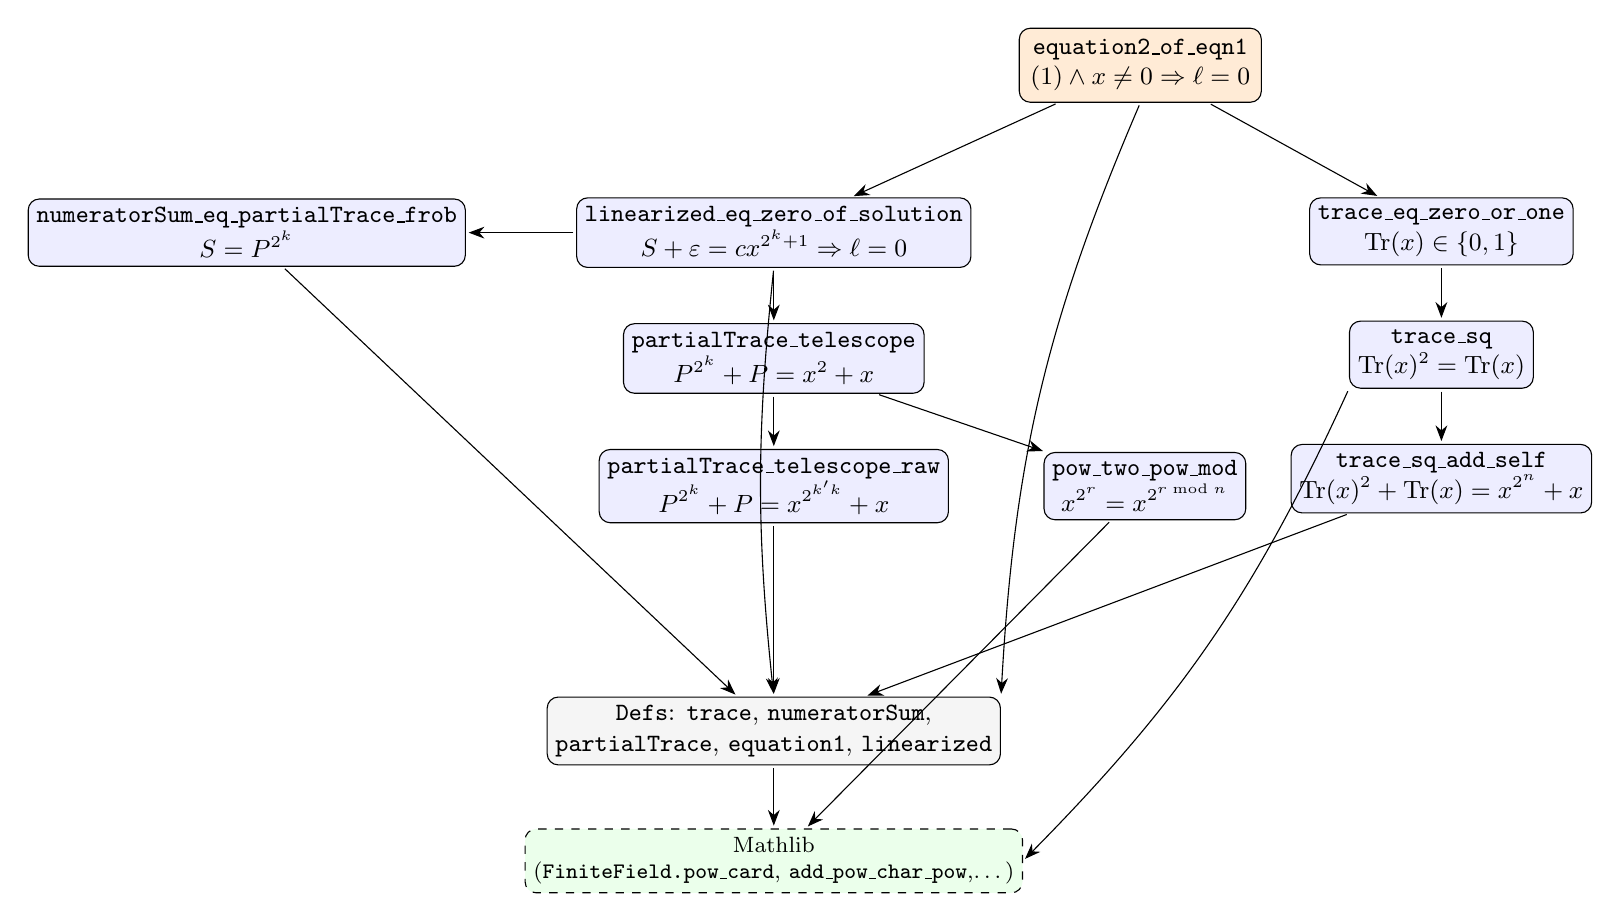
\begin{tikzpicture}[node distance=7mm and 12mm]
\node[head] (H) {\lc{equation2\_of\_eqn1}\\$(1)\wedge x\neq0\Rightarrow\ell=0$};

\node[lem,below left=12mm and 6mm of H] (LIN) {\lc{linearized\_eq\_zero\_of\_solution}\\$S+\varepsilon=c x^{2^k+1}\Rightarrow\ell=0$};
\node[lem,below right=12mm and 6mm of H] (TB) {\lc{trace\_eq\_zero\_or\_one}\\$\Tr(x)\in\{0,1\}$};

\node[lem,below=of LIN] (TEL) {\lc{partialTrace\_telescope}\\$P^{2^k}+P=x^2+x$};
\node[lem,left=14mm of LIN] (SEQ) {\lc{numeratorSum\_eq\_partialTrace\_frob}\\$S=P^{2^k}$};

\node[lem,below=of TEL] (RAW) {\lc{partialTrace\_telescope\_raw}\\$P^{2^k}+P=x^{2^{k'k}}+x$};
\node[lem,right=12mm of RAW] (FROB) {\lc{pow\_two\_pow\_mod}\\$x^{2^r}=x^{2^{r\bmod n}}$};

\node[lem,below=of TB] (TSQ) {\lc{trace\_sq}\\$\Tr(x)^2=\Tr(x)$};
\node[lem,below=of TSQ] (TSAS) {\lc{trace\_sq\_add\_self}\\$\Tr(x)^2+\Tr(x)=x^{2^n}+x$};

\node[def,below=22mm of RAW] (DEFS) {\lc{Defs}: \lc{trace}, \lc{numeratorSum},\\ \lc{partialTrace}, \lc{equation1}, \lc{linearized}};
\node[mlib,below=8mm of DEFS] (M) {Mathlib\\(\lc{FiniteField.pow\_card}, \lc{add\_pow\_char\_pow},\dots)};

\draw[ar] (H) -- (LIN);
\draw[ar] (H) -- (TB);
\draw[ar] (H.south) to[bend right=10] (DEFS.north east);
\draw[ar] (LIN) -- (TEL);
\draw[ar] (LIN) -- (SEQ);
\draw[ar] (LIN.south) to[bend right=6] (DEFS.north);
\draw[ar] (TEL) -- (RAW);
\draw[ar] (TEL) -- (FROB);
\draw[ar] (SEQ) -- (DEFS);
\draw[ar] (RAW) -- (DEFS);
\draw[ar] (FROB) -- (M);
\draw[ar] (TB) -- (TSQ);
\draw[ar] (TSQ) -- (TSAS);
\draw[ar] (TSAS) -- (DEFS);
\draw[ar] (DEFS) -- (M);
\draw[ar] (TSQ.south west) to[bend left=10] (M.east);
\end{tikzpicture}}
\end{center}

% =======================================================================
\section{Module-level DAG and the \lc{SimpleGraph} proof space}
% =======================================================================
The library is split into six modules over a common Mathlib base.  The directed
DAG (left) is transcribed \emph{verbatim} into the Lean relation \lc{dep}; its
undirected \lc{SimpleGraph} \lc{depGraph} (right) is proved \textbf{connected}.

\begin{center}
\begin{minipage}[c]{0.46\textwidth}\centering
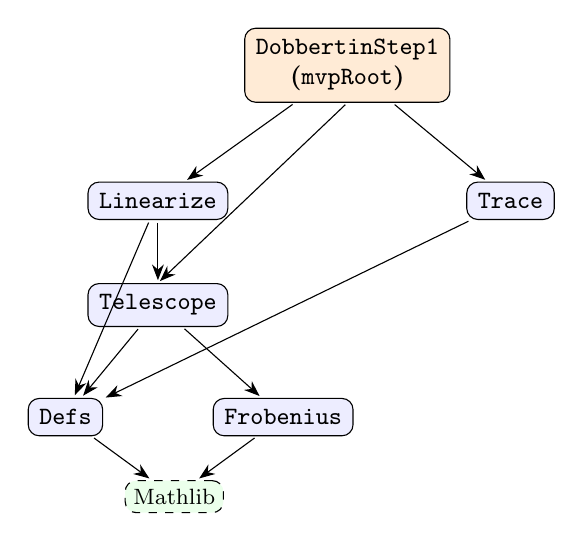
\begin{tikzpicture}[node distance=8mm and 10mm]
\node[head] (S1) {\lc{DobbertinStep1}\\(\lc{mvpRoot})};
\node[mod,below left=10mm and 2mm of S1] (LIN) {\lc{Linearize}};
\node[mod,below right=10mm and 2mm of S1] (TR) {\lc{Trace}};
\node[mod,below=of LIN] (TEL) {\lc{Telescope}};
\node[mod,below left=9mm and -2mm of TEL] (DE) {\lc{Defs}};
\node[mod,below right=9mm and -2mm of TEL] (FR) {\lc{Frobenius}};
\node[mlib,below=8mm of $(DE)!0.5!(FR)$] (M) {Mathlib};
\draw[ar] (S1) -- (LIN); \draw[ar] (S1) -- (TR);
\draw[ar] (S1.south) -- (TEL.north);
\draw[ar] (LIN) -- (TEL); \draw[ar] (LIN) -- (DE);
\draw[ar] (TR) -- (DE);
\draw[ar] (TEL) -- (DE); \draw[ar] (TEL) -- (FR);
\draw[ar] (DE) -- (M); \draw[ar] (FR) -- (M);
\end{tikzpicture}\\[2pt]
{\footnotesize directed DAG $=$ Lean \lc{dep}}
\end{minipage}\hfill
\begin{minipage}[c]{0.5\textwidth}\centering
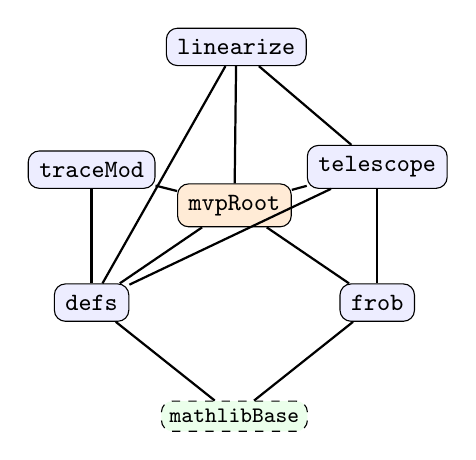
\begin{tikzpicture}[node distance=9mm and 11mm]
\node[mlib] (M) {\lc{mathlibBase}};
\node[mod,above left=10mm and 4mm of M] (DE) {\lc{defs}};
\node[mod,above right=10mm and 4mm of M] (FR) {\lc{frob}};
\node[mod,above=12mm of DE] (TR) {\lc{traceMod}};
\node[mod,above=12mm of FR] (TEL) {\lc{telescope}};
\node[mod,above left=10mm and 0mm of TEL] (LIN) {\lc{linearize}};
\node[head,above=22mm of M] (S1) {\lc{mvpRoot}};
\draw[ug] (DE) -- (M); \draw[ug] (FR) -- (M);
\draw[ug] (TR) -- (DE); \draw[ug] (TEL) -- (DE); \draw[ug] (TEL) -- (FR);
\draw[ug] (LIN) -- (DE); \draw[ug] (LIN) -- (TEL);
\draw[ug] (S1) -- (DE); \draw[ug] (S1) -- (FR); \draw[ug] (S1) -- (TR);
\draw[ug] (S1) -- (TEL); \draw[ug] (S1) -- (LIN);
\end{tikzpicture}\\[2pt]
{\footnotesize undirected \lc{depGraph} $=$ \lc{SimpleGraph.fromRel dep}}
\end{minipage}
\end{center}

\noindent In \lc{DobbertinStep1/ProofSpace.lean}:
\begin{quote}\small\ttfamily
inductive Node\\
\ \ | mathlibBase | defs | frob | traceMod | telescope | linearize | mvpRoot\\[4pt]
def dep : Node $\to$ Node $\to$ Prop \ $\ldots$\\
def depGraph : SimpleGraph Node := SimpleGraph.fromRel dep\\[4pt]
theorem reach\_mathlibBase (v : Node) : depGraph.Reachable mathlibBase v\\
theorem depGraph\_connected : depGraph.Connected
\end{quote}
The theorem \lc{depGraph\_connected} certifies that the entire proof space
collapses, through its dependency edges, onto the single \lc{mathlibBase} node:
there is no orphaned or free-floating component.

% =======================================================================
\section*{Soundness}
% =======================================================================
Every declaration in \lc{DobbertinStep1} is \lc{sorry}-free; the headline
\lc{equation2\_of\_equation1} depends only on the standard axioms
\lc{propext}, \lc{Classical.choice}, \lc{Quot.sound}.

\end{document}
